\setcounter{page}{1}
\chapter{Bitcoin}

\section{Introduction}

Bitcoin is a digital currency that uses \emph{blockchain} technology to track
and verify transactions. It was created in 2009 by an unknown individual or
group using the pseudonym \emph{Satoshi Nakamoto}.
Bitcoin is decentralized, meaning that it is not controlled by any government
or institution. Instead, it relies on a network of computers around the world
to process and verify transactions.
The technology used is known with the name blockchain, and it is a transparent
and secure record of all transactions that have
ever occurred on the network.

\section{Bitcoin Basics}
\label{sec:basics}

One of the key features of Bitcoin is its limited supply. There will only ever
be 21 million bitcoins in existence, and the rate at which new bitcoins are
created is gradually decreasing. This built-in scarcity is one of the factors
that makes Bitcoin valuable.
However, the innovative idea proposed by Bitcoin was not a virtual currency that can be
exchange on internet, but Bitcoin solves the problem of authority inside this kind
of system through a proof of work protocol that was first proposed in a paper
by Adam Back in 1997 called \quotes{Hashcash - A Denial of Service Counter-Measure}.

In the context of Bitcoin, proof of work is a system that is used to secure the
blockchain and prevent fraud. It is a mathematical algorithm that requires computers
to perform a certain amount of computational work in order to create a new
block of transactions on the blockchain.
For this reason, the core ideas that make Bitcoin a solid and sicure cryptocurrency 
is also limiting the protocol in different way, and one of these limitation is the number of
transactions that the network can process for second.

The current upper limit is around 7 transactions per second, 
which is relatively low compared to other payment systems, and 
this limtiation (that it is considered a feature) can led to congestion
on the network. 
In the April of 2022 there is the first real example of congestion 
related to the limit of transactions when the usage of bitcoin
grown disproportionately as the Figure \ref{fig:fee_x_block} shows, and this
cause an increate of the transactions fee untill the point to make 
the Bitcoin unusable for small amount.

\begin{figure}
    \begin{center}
      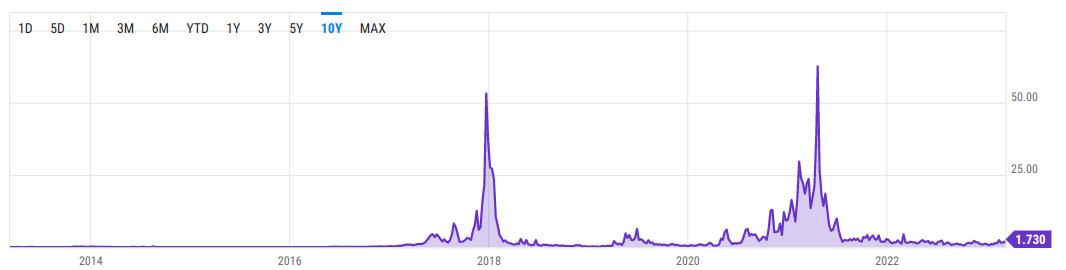
\includegraphics[scale=0.3]{imgs/feerate_blocks.png}
    \end{center}
    \caption{Fee per block in 2021.}
    \label{fig:fee_x_block}
\end{figure}


Overall, the limited number of transactions and the scalability issues on the Bitcoin network
are significant challenges that need to be addressed in order for the network to continue
to grow and evolve. There are various proposals such as \emph{Side Chain} and \emph{Lightning Network}, 
and in the Section \ref{sec:lightning_network} the Lightning Network protocol is discussed.


\section{Bitcoin Transaction}

Transactions are a fundamental part of Bitcoin. In fact, the entire system is designed to ensure
the creation, propagation, and publication of transactions on the blockchain, but these
transactions are conceptually different from the transactions we are used to.
For example, a transaction in a relational database represents an event that triggers a
change in state within the database, where in case of malfunctions, the database returns
to the previous condition before the event was triggered.
The transactions of Bitcoin are conceptually different.

In fact, the transactions are generated by a wallet, and propagated to the network
where there are special node called \emph{mainers} that collect the transactions
validate them, and build a new block that will be proposed to be stored inside 
the blockchain. During this process the miners perform the proof of work as 
describec in \cite{Palazzo_Estrazione_di_Informazioni_2021}.
Another interesting aspect of the transactions is the concept of 
Unspend Transactions Output (UTXOs), as described in \cite{Palazzo_Estrazione_di_Informazioni_2021} 
and the meccanism to spend a transaction.
A transaction is a datastucture (as the Table \ref{tab:rawtxbitcoinc} shows) that contains the core information
of Bitcoin transaction: 

\begin{table}[H]
    \centering\small
       \begin{tabular}{|c|c|}
        \hline
        \multicolumn{2}{|c|}{\textbf{RawTransaction}} \\
        \hline
        \multicolumn{1}{|c|}{Type} & \multicolumn{1}{c|}{Name} \\       
        \hline \hline
        $int32\_t$ & version   \\
        \hline
        $uint8\_t$ & marker \\
        \hline
        $uint8\_t$ & flag \\
        \hline
        CompactSize & numberTxIn \\
        \hline
        vector<TransactionInput> & transactionsInput \\
        \hline
        CompactSize & numberTxOut \\
        \hline
        vector<TransactionOutput> & transactionsOutput \\
        \hline
        vector<TransactionWitness> & transactionsWitness \\
        \hline
    \end{tabular}   
    \caption{Transaction struct\cite{Palazzo_Estrazione_di_Informazioni_2021}.\label{tab:rawtxbitcoinc}}
\end{table}

\begin{itemize}
    \item {\bf Raw Transaction}: Main transaction concept that contains the information
        regarding the transactions input and the transactions output;
    \item {\bf transactionsInput}: A transaction spend a previous transaction contained
        inside UTXOs set, and this kind of transaction are included inside
        the transaction input array;
    \item {\bf transactionsOutput}: A wallet while creating a transaction, will spend some previous
        transaction (input transaction) and generate a new transaction called \emph{output transaction}.
\end{itemize}


\begin{example}
    \label{ex:how_spend_bitcoin}
    For example, Alice want to pay Bob with bitcoin, so in order to do that Alice
    use the own UTXO to pay Bob. The wallet of Alice in this case creates a new transaction
    capable of \emph{unlock} the Alice UTXO, and at the same time the wallet create 
    a new transaction that Bob owns (that only Bob can unlock) by including this new transaction inside the transactions output array. 

    In this way now Alice consumed the UTXO that means spend bitcoins and Bob receive bitcoin by collecting UTXO that he owns. 
    If Bob want to pay Sara, he should repete the privious step and create a transaction output that Sara can own,
    and the Figure \ref{fig:lockunlockexample} shows.

    {\centering
     \vspace{5pt}
      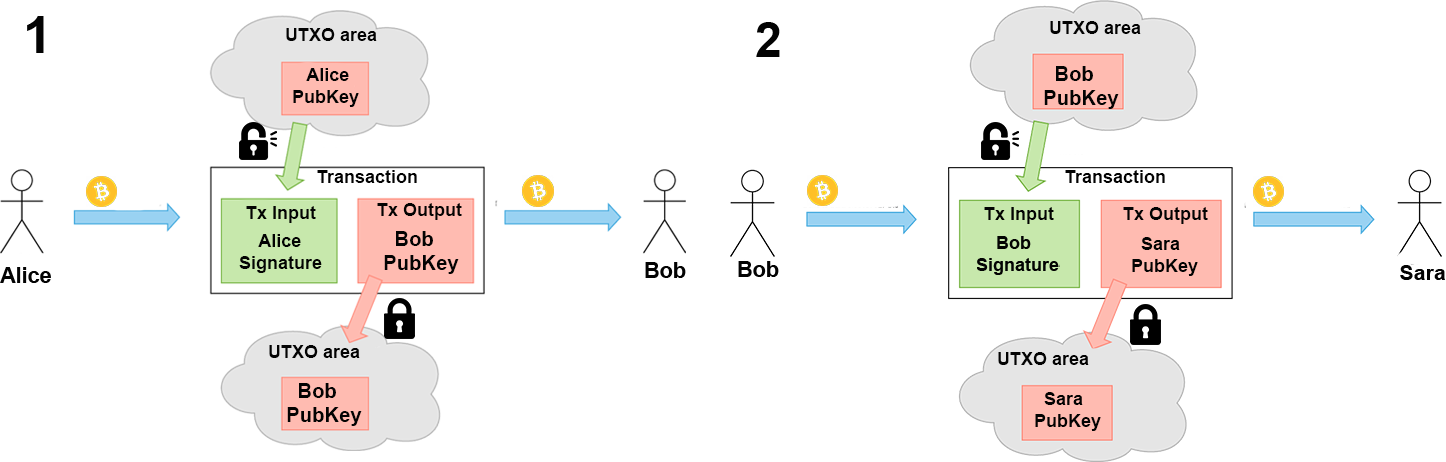
\includegraphics[scale=0.3]{imgs/DiagramUnlocLockUTXO.png}
      \captionof{figure}{UTXO usage as described inside the example.\cite{Palazzo_Estrazione_di_Informazioni_2021}\label{fig:lockunlockexample}}
      \vspace{10pt}
     \par}
\end{example}

In this section there is only a generic discussion about the transactions, and it is not take into count 
what happens it the UTXO is not consumed in total! In the paper \cite{Palazzo_Estrazione_di_Informazioni_2021}
there is a deep discussion on how the Bitcoin Transactions works.

\section{Bitcoin Script}

- Take the ownable transaction concept and introduce the bitcoin script
- Introduce an example that can be evolved long all the paper.

At the core of Bitcoin Protocol there is a concept of transaction, and it is used to transfer value
between users on the network. When a user is identified by a private and public wants, and the own of a
Bitcoin transaction is expressed in the he possibility to unlock a Unspendable transaction output.

The Bitcoin protocol do not express any concept of Bitcoin account, but there is a concept of address
derived from a \emph{Bitcoin script} program encoded inside the transaction.

A Bitcoin script is a simple, stack-based programming language used to encode the rules for a specific
transaction or set of transactions on the Bitcoin network. Scripts are used to determine how the
funds in a particular transaction can be spent, as well as to enforce certain rules on the network such as the owners
of the bitcoin transactions.

\subsection{Bitcoin Script Basics}

- Bitcoin Script basics, introduce how the bitcoin scrips works, and how may
kind of scripts exists
- Introduce the Bitcoin no standard
- Make a small zoom of what happens with the Bitcoin Script inside the example
